% !TEX TS-program = pdflatex
% !TEX encoding = UTF-8 Unicode

% This is a simple template for a LaTeX document using the "article" class.
% See "book", "report", "letter" for other types of document.

\documentclass[11pt]{article} % use larger type; default would be 10pt

\usepackage[utf8]{inputenc} % set input encoding (not needed with XeLaTeX)

%%% PAGE DIMENSIONS
\usepackage{geometry} % to change the page dimensions
\geometry{a4paper} % or letterpaper (US) or a5paper or....

\usepackage{graphicx} % support the \includegraphics command and options

\usepackage{amssymb}
\usepackage{amsmath}
%%% PACKAGES
\usepackage{booktabs} % for much better looking tables
\usepackage{array} % for better arrays (eg matrices) in maths
\usepackage{paralist} % very flexible & customisable lists (eg. enumerate/itemize, etc.)
\usepackage{verbatim} % adds environment for commenting out blocks of text & for better verbatim
\usepackage{subfig} % make it possible to include more than one captioned figure/table in a single float
% These packages are all incorporated in the memoir class to one degree or another...

%%% HEADERS & FOOTERS
\usepackage{fancyhdr} % This should be set AFTER setting up the page geometry
\pagestyle{fancy} % options: empty , plain , fancy
\renewcommand{\headrulewidth}{0pt} % customise the layout...
\lhead{}\chead{}\rhead{}
\lfoot{}\cfoot{\thepage}\rfoot{}

%%% SECTION TITLE APPEARANCE
\usepackage{sectsty}
\allsectionsfont{\sffamily\mdseries\upshape} % (See the fntguide.pdf for font help)
% (This matches ConTeXt defaults)

%%% ToC (table of contents) APPEARANCE
\usepackage[nottoc,notlof,notlot]{tocbibind} % Put the bibliography in the ToC
\usepackage[titles,subfigure]{tocloft} % Alter the style of the Table of Contents
\renewcommand{\cftsecfont}{\rmfamily\mdseries\upshape}
\renewcommand{\cftsecpagefont}{\rmfamily\mdseries\upshape} % No bold!

\usepackage{hyperref}
\usepackage{amsmath}
\usepackage{graphicx}
\graphicspath{ {./pings/} }
\DeclareMathOperator*{\argmax}{arg\,max}
\DeclareMathOperator*{\argmin}{arg\,min}

\newcount\colveccount
\newcommand*\colvec[1]{
        \global\colveccount#1
        \begin{pmatrix}
        \colvecnext
}
\def\colvecnext#1{
        #1
        \global\advance\colveccount-1
        \ifnum\colveccount>0
                \\
                \expandafter\colvecnext
        \else
                \end{pmatrix}
        \fi
}

%%% END Article customizations

%%% The "real" document content comes below...

\title{Micro HW1}
\author{Michael B. Nattinger\footnote{I worked on this assignment with my study group: Alex von Hafften, Andrew Smith, Ryan Mather, and Tyler Welch. I have also discussed problem(s) with Emily Case, Sarah Bass, Katherine Kwok, and Danny Edgel.}}

%\date{} % Activate to display a given date or no date (if empty),
         % otherwise the current date is printed 

\begin{document}
\maketitle

\section{Question 1}
\subsection{Part A}
The game consists of players $I = \{ 1,\dots,N\}$. Each player is of type $\theta \sim  F$. Each player plays a strategy $b:[0,1]\rightarrow \mathbb{R}$ which is a function of their type. The a priori belief is that everyone's type is drawn from $F$. The interim belief is full knowledge of one's own type, and knowing that everyone else's type is drawn from $F$. The ex ante belief is full knowledge of all types. The person with the highest bid wins the auction and thus gains their valuation, and all players (including the winner) pays their bid regardless of winning or losing.
\subsection{Part B}
Each player faces the following utility maximization problem:
\begin{align*}
\max_{b_i} E[U(b_i)]\\
\max_{b_i} \theta_i Pr(b_i>\max_{j\neq i}\{b_{j}\}) - b
\end{align*}
In our case, with $iid$ observations, $Pr(b_i>\max_{j\neq i}\{b_{j}\}) = \Pi_{j\neq i}Pr(b_i>b_{j})$. We can also now plug in the strategy of the other players as a function. Our maximization problem now takes the following form, where $\theta_{-i}$ is any draw from $F$: 

\begin{align*}
\max_{b_i} \theta_i (Pr(b_i>b(\theta_{-i})))^{N-1} - b_i\\
\max_{b_i} \theta_i (Pr(b^{-1}(b_i)>\theta_{-i}))^{N-1} - b_i \\
\max_{b_i} \theta_i (b^{-1}(b_i))^{aN-a} - b_i
\end{align*}

Taking first order conditions,
\begin{align*}
1 &= \theta_i(aN-a) (b^{-1}(b_i))^{aN-a-1}\frac{1}{b'(b^{-1}(b_i))}\\
&= \frac{ (aN-a) (\theta_i)^{aN-a}}{b'(\theta_i))}\\
b'(\theta_i) &= (aN-a) (\theta_i)^{aN-a}\\
\Rightarrow b(\theta_i) &= \frac{aN-a}{aN-a+1}(\theta_i)^{aN-a+1} + c_{\theta_i}
\end{align*}
Players with a valuation of $0$ will bid $0$ so $c_{\theta_i}=0$. Therefore, $ b(\theta_i) = \frac{aN-a}{aN-a+1}(\theta_i)^{aN-a+1}$
%Each player will bid such that their expected payoff is $0$:
%\begin{align*}
%b(\theta) &= \theta Pr(b_i>\max_{j\neq i}\{b_{j}\})\\
%&= \theta \Pi_{j\neq i}Pr(b_i>b_{j}) \\
%&= \theta \Pi_{j\neq i}Pr(\theta_i>\theta_{j}) \\
%&= \theta (\theta^a )^{N-1}\\
%&= \theta^{1+aN-a}.
%\end{align*}
\subsection{Part C}
We can verify by rewriting the optimization problem as we did originally with the known function $b$ and show that the best reply is to follow said function.
\begin{align*}
\max_{b_i} \theta_i (Pr(b_i > b(\theta_{-i})))^{N-1} - b_i\\
\max_{b_i} \theta_i (Pr(b_i >  \frac{aN-a}{aN-a+1}(\theta_{-i})^{aN-a+1}))^{N-1} - b_i\\
\max_{b_i} \theta_i (Pr(\left(\frac{aN-a+1}{aN-a}b_i\right)^{\frac{1}{aN-a+1}} > \theta_{-i})^{N-1} - b_i\\
\max_{b_i} \theta_i \left(\frac{aN-a+1}{aN-a}b_i\right)^{\frac{aN-a}{aN-a+1}}  - b_i\\
\end{align*}
Taking FOCs:
\begin{align*}
1 &= \theta_i \frac{aN-a}{aN-a+1} \left(\frac{aN-a+1}{aN-a}b_i\right)^{\frac{aN-a}{aN-a+1} - 1}\frac{aN-a+1}{aN-a}\\
\left(\frac{aN-a+1}{aN-a}b_i\right)^{\frac{1}{aN-a+1}} &= \theta_i \\
b_i &=  \frac{aN-a}{aN-a+1}(\theta_i)^{aN-a+1} 
\end{align*}
Therefore , $b(\theta) =  \frac{aN-a}{aN-a+1}(\theta)^{aN-a+1}$ is a best response to the other players playing the same strategy. Thus, it constitutes an equilibrium.
\subsection{Part D}
As $a$ increases, bids will shrink for given types less than 1, so the bidding will become less competitive for a given type. Intuitively, as $a$ rises, more of the distribution mass is near $1$ so for a fixed $\theta$ value less than one the odds of winning decrease, and therefore the bid decreases. There is also a second effect here. For very low values of $a$, the probability of having a competitor with the same or higher valuation is very small, so by increasing $a$ marginally over low values of $a$ the likelihood of having a competitor near the value near your own fixed $\theta$ value rises, so your bid increases to reflect this increased competitveness of others relative to your type. To summarize, over very low values of $a$ the bids increase with a, but for all other $a$ values the bids are decreasing in $a$.
\subsection{Part E}

Before drawing a type, the expected bid is the following:
\begin{align*}
E[b_i(\theta)] &= \int_{0}^{1} \frac{aN-a}{aN-a+1}(\theta)^{aN-a+1}  a\theta^{a-1} d\theta \\
&=  \frac{a(aN-a)}{aN-a+1} \int_{0}^{1}\theta^{aN}d\theta\\
&=   \frac{a(aN-a)}{aN-a+1}\frac{1}{(aN+1)} 
\end{align*}

I originally interpreted the question as being the expected return of the bidder before and after drawing the type. This is not what the question asks but I still have it below.

After drawing a type, person $i$ with type $\theta_i \sim F$ bids $b(\theta_i) =  \frac{aN-a}{aN-a+1}(\theta_i)^{aN-a+1}$ and wins payoff $\theta_i$ with some probability:
\begin{align*}
E[\pi|\theta] &= \theta_i Pr(\theta_i>\theta_{-i})^{N-1} - b(\theta_i)\\
&= \theta_i^{aN-a+1} - \frac{aN-a}{aN-a+1}(\theta_i)^{aN-a+1}\\
&= \frac{1}{aN - a + 1}\theta_i^{aN-a+1}
\end{align*}

We can find the expected winnings prior to drawing a type by taking the expectation of winnings by type across the distribution of types. Note that $F(\theta) = \theta^a \Rightarrow f(\theta) = a\theta^{a-1}$. Then, we have the following:
\begin{align*}
E[\pi] &= \int_{0}^1 E[\pi|\theta] f(\theta)d\theta \\
&=  \int_{0}^1\frac{1}{aN - a + 1}\theta^{aN-a+1} a\theta^{a-1}d\theta\\
&= \frac{a}{aN - a + 1}\int_{0}^1\theta^{aN} d\theta\\
&=  \frac{a}{aN - a + 1} \frac{1}{aN+1}.
\end{align*}
\section{Question 2}
\subsection{Part A}
Suppose there exists bidding strategies $b_1(x),b_2(x)$ for individuals $F_1(x) = x,F_2(x) = x^2$ which are known to all individuals and form an equilibrium (non-symmetric due to non-iid types). The payoff for person 1 is then the following:
\begin{align*}
(x_1-b_1)Pr(b_1>b_2(x_2)) &= (x_1-b_1)(b_2^{-1}(b_1))^2
\end{align*}

Taking FOCs wrt $b_1$:
\begin{align*}
\frac{2(x_1 - b_1)b_2^{-1}(b_1)}{b_2'(b_2^{-1}(b_1))}-(b_2^{-1}(b_1))^2 &= 0
\end{align*}
\begin{align}
b_1(x_1) &= x_1 - (1/2)b_2'(b_2^{-1}(b_1(x_1)))(b_2^{-1}(b_1(x_1)))  \label{de1}
\end{align}

The payoff for person 2 is then the following:
\begin{align*}
(x_2-b_2)b_1^{-1}(b_2)
\end{align*}

Taking FOCs wrt $b_2$:
\begin{align*}
\frac{(x_2 - b_2)}{b_1'(b_1^{-1}(b_2))}-b_1^{-1}(b_2) &= 0
\end{align*}

\begin{align}
b_2(x_2) &= x_2 - b_1'(b_1^{-1}(b_2(x_2)))b_1^{-1}(b_2(x_2)) \label{de2}
\end{align}

$b_1,b_2$ are equilibrium bidding strategies which satisfy the differential equations (\ref{de1}),(\ref{de2}). They also satisfy the fact that $b_1(r) = r = b_2(r)$, as agents who draw type $r$ should receive no surplus. These form the boudary conditions on the differential equations. We cannot solve analytically, but we can solve numerically. Note that the fact that these equations are positive and (strictly) increasing implies that both bidders bid below their valuations, which can be seen directly in equations (\ref{de1}),(\ref{de2}).
\subsection{Part B}
In the second-price auction, both people will bid their valuations - we saw in class that the strategy was weakly dominant in the second price auction without reserve price, and the same logic holds here. If both bids are above $r$, then the seller with the higher bid will pay the seller the second-highest price, and will receive the object. If one valuation is above $r$ then that individual will pay $r$ and receive the object. If both valuations are below $r$ then no trade will occur.
\subsection{Part C}
The revenue equivalence theorem does not hold here as the agents are drawn from different distributions, and the type $2$ agent is more likely to win as their type distribution first order stochastically dominates the type 1 agent. We can find the optimal $r$ to pick for both types of auction, and then calculate the revenue at the optimums and compare the two types of auctions.

First we will maximize profit of the first-price auction. The highest type will win conditional on having a type above $r$:
\begin{align*}
\pi^1 &= E[b_1(x_1) - c| b_1(x_1)>r>b_2(x_2)]P(b_1(x_1)>r>b_2(x_2)) \\&+ E[b_1(x_1) - c|b_1(x_1)>b_2(x_2)>r]P(b_1(x_1)>b_2(x_2)>r) \\&+ E[b_2(x_2) - c|b_2(x_2)>r>b_1(x_1) ]P(b_2(x_2)>r>b_1(x_1)) \\&+ E[b_2(x_2) - c|b_2(x_2)>b_1(x_1)>r ]P(b_2(x_2)>b_1(x_1)>r)\\
%&= E\left[ \frac{2}{3}x_1 + \frac{r^3}{3x_1^2} - c| x_1>r\right]P(x_1>r>x_2) + E\left[ \frac{2}{3}x_1 + \frac{r^3}{3x_1^2}- c| x_1>x_2>r\right]P(x_1>x_2>r) \\&+ E\left[ \frac{x_2^2 + r^2}{2x_2}  - c|x_2>r\right]P(x_2>r>x_1) + E\left[ \frac{x_2^2 + r^2}{2x_2} - c|x_2>x_1>r \right]P(x_2>x_1>r)\\
%&= \left( \int_{r}^1 \frac{2}{3}x + \frac{r^3}{3x^2} dx - c \right)\int_{r}^1\int_{0}^r 2x_2 dx_2dx_1 \\&+\left(\int_r^1\int_{r}^{x_1} 2x_2dx_2\left( \frac{2}{3}x_1 + \frac{r^3}{3x_1^2}\right) dx_1- c\right) \int_{r}^1\int_{r}^{x_1} 2x_2 dx_2dx_1  \\&+ \left( \int_{r}^1 x^2 + r^2 dx - c \right)\int_{r}^1\int_{0}^r  dx_1 2x_2 dx_2 + \left(\int_r^1\int_{r}^{x_2}  dx_1\left( x_2^2 + r^2\right)dx_2- c\right) \int_{r}^1\int_{r}^{x_2}  dx_1 2x_2 dx_2\\
%&= \left( \frac{1}{3}(1-r^3) - c \right)(r^2-r^3) + \left( \frac{1}{6}(1-r)^2(2r^3 + r^2 + 2r +1) - c \right)\left( \frac{1}{3}(1-r)^2(2r+1)\right) \\
%&+ \left(r^2 -\frac{4}{3}r^3 +\frac{1}{3} - c \right)(r-r^3) + \left(\frac{1}{12}(1-r)^2(7r^2+2r+3)  - c \right)\frac{1}{3}\left( r^3 - 3r + 2 \right)
\end{align*}
$r^{1*}$ satisfies the first order condition of the above expression with respect to $r$. I will solve computationally. Then, maximum profits can be computed as a function of c.

Next we will maximize profit of the second-price auction. 
\begin{align*}
\pi^2 &=  E[r - c| x_1>r>x_2]P(x_1>r>x_2) + E[x_2 - c| x_1>x_2>r]P(x_1>x_2>r) \\&+ E[r - c|x_2>r>x_1 ]P(x_2>r>x_1) + E[x_1 - c|x_2>x_1>r ]P(x_2>x_1>r) \\
&= (r - c)\int_{r}^1\int_{0}^r 2x_2 dx_2dx_1+ \left( \int_{r}^1 \int_r^{x_1}2x_2^2 dx_2 dx_1 - c \right) \int_{r}^1\int_{r}^{x_1} 2x_2 dx_2dx_1 \\&+ (r - c)\int_{r}^1\int_{0}^r  dx_1 2x_2 dx_2 + \left( \int_{r}^1 \int_r^{x_2}2x_2x_1 dx_1 dx_2 - c \right)\int_{r}^1\int_{r}^{x_2}  dx_1 2x_2 dx_2 \\
&= (r-c)(r^2-r^3) + \left(\frac{1}{6}(3r^4 - 4r^3 + 1) - c \right) \left( \frac{1}{3}(r-1)^2(2r+1) \right) \\ &+ (r-c)(r-r^3) + \left(\frac{1}{4}(r^2-1)^2 - c\right)
\frac{1}{3}(r^3 - 3r + 2)\end{align*}
$r^{2*}$ satisfies the first order condition of the above expression with respect to $r$. I will solve computationally. Then, maximum profits can be computed as a function of c. We can then compare to the first price auction.

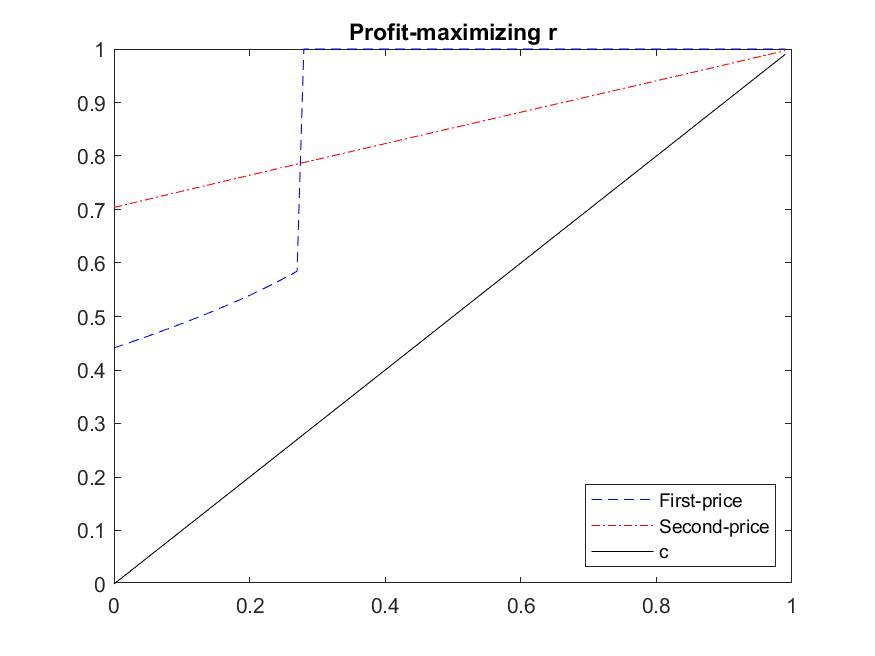
\includegraphics{argmax}

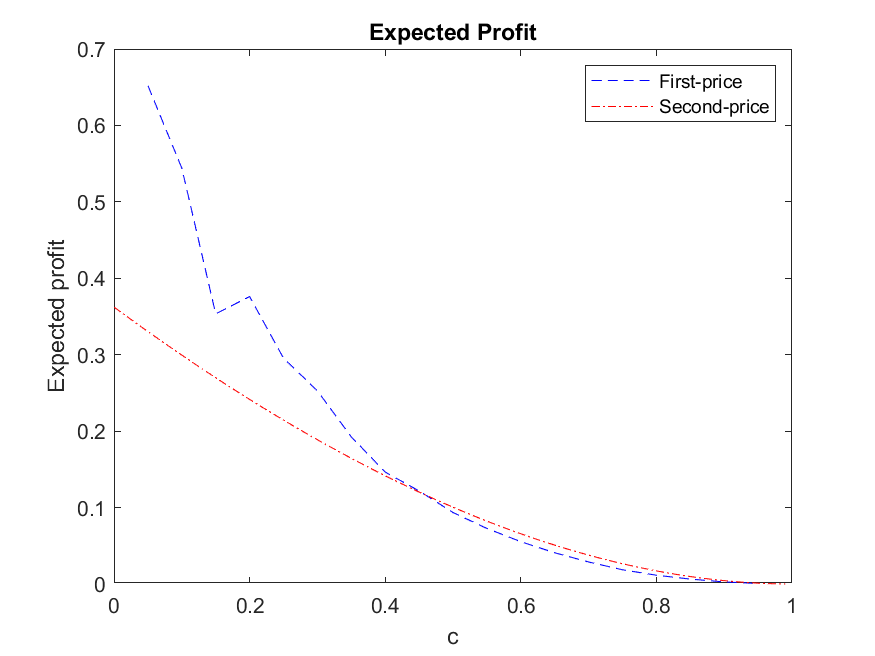
\includegraphics{profit}

We can see from the above figures that the profit-maximizing seller will choose the second price auction as they receive weakly higher profit for $c\in [0,1]$.

\subsection{Part D}
The discount should be offered to the type that tends to have the lowest valuation $F(x) = x$. The idea is to try to get them to bid over their valuation, while staying the second-highest bidder, raising the sale price of the good. We calculate the optimal discount.

The type that receives the discount will bid such that they would receive no surplus buying the item at that price: $\alpha b - x = 0\Rightarrow b = \frac{x}{\alpha}$. The other type bids their valuation. The seller chooses $\alpha$ to maximize expected revenue:

\begin{align*}
&\max_{\alpha} E\left[\frac{x_1}{\alpha}|\frac{x_1}{\alpha}<x_2\right] P\left(\frac{x_1}{\alpha}<x_2\right) + E\left[x_2|\frac{x_1}{\alpha}>x_2\right] P\left(\frac{x_1}{\alpha}>x_2\right)\\
&\max_{\alpha} \frac{1}{\alpha}\int_{0}^1\int_{0}^{\alpha x_2} x_1 dx_1 2x_2 dx_2 \int_{0}^1\int_{0}^{\alpha x_2} dx_1 2x_2 dx_2 + \int_{0}^1\int_{0}^{x_1/\alpha} 2x_2^2 dx_2 dx_1 \int_{0}^1\int_{0}^{x_1/\alpha}2x_2 dx_2  dx_1 \\
&\max_{\alpha} 2\alpha^2\int_{0}^1 x_2^3  dx_2 \int_{0}^1 x_2^2 dx_2 + \frac{2}{3\alpha^5}\int_{0}^1 x_1^3 dx_1 \int_{0}^1 x_1^2 dx_1 \\
&\max_{\alpha} \frac{\alpha^2}{6}+ \frac{1}{18\alpha^5} 
\end{align*}
Taking FOCs:
\begin{align*}
\frac{\alpha}{3} &= \frac{5}{18\alpha^6}\\
\alpha^7 &= \frac{5}{6}\\
\alpha &= \left( \frac{5}{6} \right)^{1/7}.
\end{align*}

Using this discount value, the expected revenues are the following:
\begin{align*}
ER &=  \frac{\alpha^2}{6}+ \frac{1}{18\alpha^5} \\
&= \frac{1}{6}\left( \frac{5}{6} \right)^{2/7} + \frac{1}{18}\left( \frac{5}{6} \right)^{-6/7}\\
&= 0.206.
\end{align*}

Note that we can make more profits by instead setting an optimal reserve price as in part C - since $c=0$, $r^{*} \approx 0.7$ yields the maximum profit of $\approx 0.36>0.206$.

\section{Question 3}
\subsection{Part A}
The game consists of players $I = \{ 1,2,3\}$. Each player is of type $v \sim  [0,1]$. Each player plays a strategy $b:[0,1]\rightarrow \mathbb{R}$ which is a function of their type. The a priori belief is that everyone's type is drawn from $[0,1]$. The interim belief is full knowledge of one's own type, and knowing that everyone else's type is drawn from $[0,1]$. The ex ante belief is full knowledge of all types. The person with the highest bid wins the auction and thus gains their valuation, and that player pays the lowest bid.
\subsection{Part B}
Player $i\in I$ maximizes their expected value. We will assume that  players $-i$ play the strategy $b(v) = \frac{n-1}{n-2}v $, then prove that the best response is the same strategy.

The optimization problem is the following:
\begin{align*}
%\max_{b_i} (v_i - \frac{n-1}{n-2}\min_{j \neq i}v_j)Pr(b_i>\frac{n-1}{n-2}\max_{j\neq i} v_j)\\
%\max_{b_i} (v_i - \frac{n-1}{n-2}\min_{j \neq i}v_j)Pr(b_i>\frac{n-1}{n-2}v_{-i})^2\\
%\max_{b_i} (v_i - \frac{n-1}{n-2}\min_{j \neq i}v_j)(b_i\frac{n-2}{n-1})^{n-1}
\max_{b_i}E[v_i - \frac{n-1}{n-2}\text{second}_{j \neq i}v_j|b_i>\frac{n-1}{n-2}\max_{j\neq i} v_j]Pr(b_i>\frac{n-1}{n-2}\max_{j\neq i} v_j) 
\end{align*}

\begin{align*}
Pr(b_i>\frac{n-1}{n-2}\max_{j\neq i} v_j) &= Pr\left(b_i>\frac{n-1}{n-2}v_{-i}\right)^{n-1}\\
&= \left(b_i\frac{n-2}{n-1}\right)^{n-1}\\
E[v_i - \frac{n-1}{n-2}\text{second}_{j \neq i}v_j|b_i>\frac{n-1}{n-2}\max_{j\neq i} v_j]  &= E[v_i - \frac{n-1}{n-2}\text{second}_{j \neq i}v_j|\frac{n-2}{n-1}b_i>v_{j}, j\neq i ] \\
&= v_i - \frac{n-1}{n-2}E[\text{second}_{j \neq i}v_j|\frac{n-2}{n-1}b_i>v_{j}, j\neq i ]
\end{align*}

This conditional expectation is equivalent to the expectation of the second largest of $n-1$ draws from the uniform distribution $U\left(0,\frac{n-2}{n-1}b_i\right)$. The expectation of this is the expectation of the second largest of $n-1$ draws from a standard uniform distribution, scaled by $\frac{n-2}{n-1}b_i$. This expectation is, therefore, $\frac{n-2}{n-1}b_i \frac{n-2}{n}$.\footnote{See \href{https://www2.stat.duke.edu/courses/Spring12/sta104.1/Lectures/Lec15.pdf}{these lecture slides} from Duke which contain formulas from which the expectation of the $k$th order statistic of a standard uniform can be constructed. Specifically, slides 8 and 11.} We then have the following maximization problem:
\begin{align*}
\max_{b_i} v_i \left(b_i\frac{n-2}{n-1}\right)^{n-1} - \frac{n-1}{n-2} \frac{(n-2)^2}{n-1} \frac{b_i}{n} \left(b_i\frac{n-2}{n-1}\right)^{n-1}\\
\max_{b_i} v_i \left(b_i\frac{n-2}{n-1}\right)^{n-1} -   \frac{n-2}{n} b_i^n\left(\frac{n-2}{n-1}\right)^{n-1}\\
\end{align*}
Taking FOCs:
\begin{align*}
(n-1)v_ib_i^{n-2}\left(\frac{n-2}{n-1}\right)^{n-1} &= (n-2)b_i^{n-1}\left(\frac{n-2}{n-1} \right)^{n-1}\\
\Rightarrow b_i &= \frac{n-1}{n-2}v_i
\end{align*}
Thus, the best response to the other players playing $b(v_i) = \frac{n-1}{n-2}v_i$ is also to play $(v_i) = \frac{n-1}{n-2}v_i$, so the bid function $b$ is a symmetric Bayes-Nash equilibrium of the third-price auction.

\subsection{Part C}
The expected revenue of the seller is the expectation of the third largest bid:
\begin{align*}
R^3 &= E[\text{third}_{i\in I} b_i]\\
&= E[\text{third}_{i\in I}  \frac{n-1}{n-2}v_i]\\
&=  \frac{n-1}{n-2}E[\text{third}_{i\in I}  v_i]\\
&=  \frac{n-1}{n-2}\frac{n-2}{n+1}\\
&= \frac{n-1}{n+1}.
\end{align*}
\subsection{Part D}
We know from class that for $k =1$ the equilibrium strategy is to underbid and for $k=2$ the equilibrium strategy is to bid the valuation. For $k=3$ we showed above that the equilibrium strategy is to overbid. As $k$ continues to increase above $3$, the equilibrium strategy is to overbid by an increasing amount. One can show that $b^k_i(v_i) = \frac{n-1}{n-k+1}$ is the equilibrium strategy for the $k$'th price auction. I do this below:

\begin{align*}
\max_{b_i}E[v_i - \frac{n-1}{n-k+1}\text{k-1'th}_{j \neq i}v_j|b_i>\frac{n-1}{n-k+1}\max_{j\neq i} v_j]Pr(b_i>\frac{n-1}{n-k+1}\max_{j\neq i} v_j)  \\ %
\max_{b_i}(v_i - \frac{n-1}{n-k+1}E[\text{k-1'th}_{j \neq i}v_j|b_i>\frac{n-1}{n-k+1}\max_{j\neq i} v_j])\left(b_i\frac{n-k+1}{n-1}\right)^{n-1} \\
\max_{b_i}(v_i - \frac{n-1}{n-k+1}\frac{n-k+1}{n-1} b_i \frac{n-k+1}{n})\left(b_i\frac{n-k+1}{n-1}\right)^{n-1}\\
\max_{b_i}v_i\left(b_i\frac{n-k+1}{n-1}\right)^{n-1} -  b_i \frac{n-k+1}{n}\left(b_i\frac{n-k+1}{n-1}\right)^{n-1}
\end{align*}

Taking FOCs:
\begin{align*}
(n-1)v_ib_i^{n-2}\left(\frac{n-k+1}{n-1}\right)^{n-1} &= b_i^n (n-k+1)\left(\frac{n-k+1}{n-1}\right)^{n-1}\\
\Rightarrow b_i &=\frac{n-1}{n-k+1}v_i .
\end{align*}
Therefore, $b^k_i(v_i) = \frac{n-1}{n-k+1}$ is the equilibrium strategy for the $k$'th price auction.
\end{document}
